%Escrita científica - 2. Organização do paper: Introdução. Métodos. 

\section{Como escrever a Introdução}

\subsection{Características da seção}

%%
\begin{frame}{Anatomia da introdução}
\begin{figure}
\centering
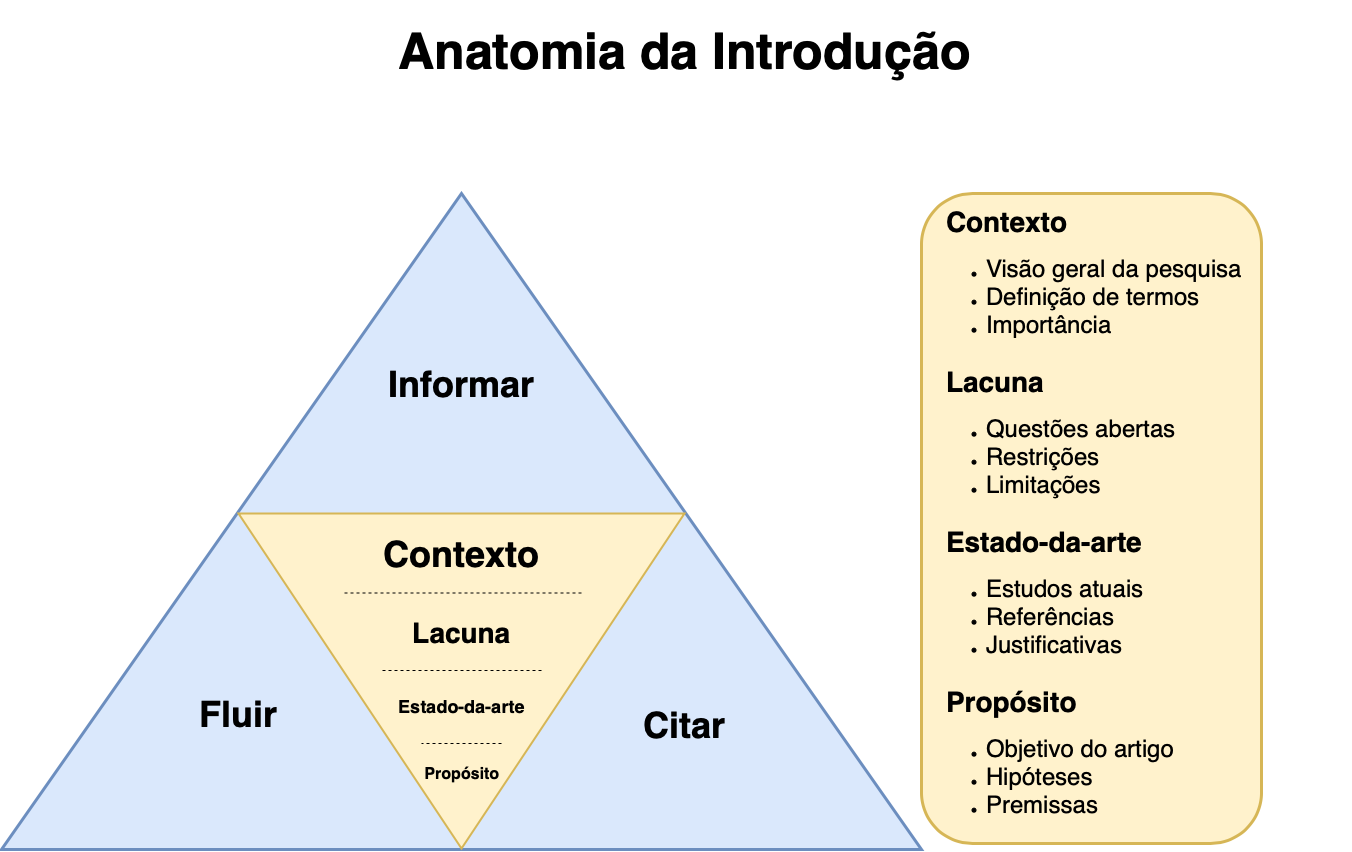
\includegraphics[scale=0.2]{figs/06/introducao-paper}
\caption{Dimensões da introdução. Baseado em (Zucolotto, 2011). Fonte: Autor.}
\end{figure}
\end{frame}

\begin{frame}{Dimensões externas da introdução}
\begin{enumerate}
\item Informação: mostre o escopo amplo onde seu assunto se insere e por que é relevante
\item Fluidez: organize o texto para que flua naturalmente estreitando-se do ``geral'' ao ``específico''
\item Citação: use referências para enfocar as idéias que os autores tiveram, não para contar um histórico do assunto ao longo do tempo
\begin{itemize}
\item Cite os artigos seminais (contexto/lacunas) 
\item Em seguida, os artigos mais recentes (estado-da-arte/lacunas)
\item Por fim, os artigos mais importantes (relevância/motivação/importância)
\end{itemize}
\end{enumerate}
\end{frame}

\begin{frame}{Dimensões internas da introdução}
\begin{enumerate}
\item Contexto: onde o estudo se aplica
\item Lacuna(s): o que não fizeram ou faltou fazer
\item Estado-da-arte: o que estão fazendo 
\item Propósito: o que você fará para contribuir
\end{enumerate}
\end{frame}


\subsection{Exercício in-class}

%%
\begin{frame}{Tarefas}
\begin{enumerate}
\item Formem 5 grupos e selecionem 1 líder por grupo
\item Cada grupo escolherá um dos artigos da lista a seguir para análise
\item Cada grupo deverá identificar, na seção \textbf{Introdução} do artigo, de 1 a 3 trechos (ou mais, se identificável) que correspondam às dimensões internas: contexto; lacunas; estado-da-arte; propósito
\item Cada líder anotará a contribuição de seu grupo em uma lista
\item Façam um rodízio dos artigos e repitam a análise 
\item No final, verificaremos se as análises convergem/divergem
\end{enumerate}
\end{frame}

\begin{frame}{Lista dos artigos} 
\begin{itemize}
\item Li2019-AdvEnMat, \url{ https://doi.org/10.1002/aenm.201902104}
\item Svane2019-ActaCrys, \url{https://doi.org/10.1107/S205327331900799X}
\item Jain2018-IEEESustEn, \url{https://doi.org/10.1109/TSTE.2018.2869480}
\item Kissas2020-CMAME,  \url{https://doi.org/10.1016/j.cma.2019.112623}
\item Jeong2019-IJHMT,  \url{https://doi.org/10.1016/j.ijheatmasstransfer.2019.118644}
\end{itemize}
\end{frame}


\subsection{Análises}

\subsubsection*{Li2019-AdvEnMat}

%%
\begin{frame}{Li2019-AdvEnMat} 
\begin{block}{Contexto}
\emph{``(...) aggravated \textbf{global energy and environmental issues} bring tremendous challenges to  the \textbf{normal functioning of modern society}.''}

\emph{``(...) a representative example is the \textbf{solar-to-hydrogen fuel conversion via water splitting} (...) ''}
\end{block}
\end{frame}

%%
\begin{frame}{Li2019-AdvEnMat} 
\begin{block}{Lacunas}
\emph{``(...) these processes are of \textbf{sluggish kinetics} and \textbf{require robust electrocatalysts to boost the reaction rates}.''}

\emph{``(...) practical applications are surely \textbf{constrained by their high cost and limited availability}.''}

\emph{``it is of great significance \textbf{to find cheap and efficient electrocatalysts} with the aim of \textbf{making these promising energy-related technologies commercially viable}.}''
\end{block}
\end{frame}

\begin{frame}{Li2019-AdvEnMat} 
\begin{block}{Estado-da-arte}
\scriptsize{
\emph{``(...) the search for electrocatalysts was \textbf{relied on trials and errors}[7]''}

\emph{``(...) an \textbf{early study indicated} that MoS2 was nonreactive toward hydrogen evolution reaction (HER)...[5b,10]''}

\emph{``The first catalytic applications of TMPs can be dated back to the 1980s \textbf{when some TMPs presented the remarkable catalytic performance} in hydrodesulfurization (HDS)....[25] ''}

\emph{``In the past few years, earth-abundant transition metal dichal-cogenides (TMDs),[16b] metal oxides (TMOs),[14a] metal carbides (TMCs),[35] metal nitrides (TMNs),[36] and pure metals (TMs) have also emerged as catalysts''}
} % close
\end{block}
\end{frame}

%%
\begin{frame}{Li2019-AdvEnMat} 
\begin{block}{Propósito}
\emph{``(...) we aim to provide an in-depth understanding of the theory-structure-function relationship and offer the unequivocal reasons behind the improved electrocatalytic performance.''}

\emph{``(...) remaining challenges and outlooks are clarified to offer a fresh impetus for designing robust TMPs electrocatalysts.''}
\end{block}
\end{frame}

\subsubsection*{Svane2019-ActaCrys}

%%
\begin{frame}{Svane2019-ActaCrys} 
\begin{block}{Contexto}
\emph{``Detailed knowledge of the \textbf{nature of chemical bonding is a prerequisite for understanding the physical and chemical properties of materials}, and experimentally this information is best available in the electron density (ED).''}
\end{block}
\end{frame}

%%
\begin{frame}{Svane2019-ActaCrys} 
\begin{block}{Lacunas}
\emph{``Improper correction for these effects gives rise to \textbf{systematic errors} in the collected data, which \textbf{reduce the quality of the obtained ED distributions} as well as ADPs. (...)''}

\emph{``These systematic \textbf{errors are essentially avoided in a powder X-ray diffraction (PXRD) measurement}.''}

\emph{``\textbf{A further complication for molecular crystals lies in the deconvolution of ED deformation}, atomic positions and ADPs, as these features correlate to a high extent (Bindzus et al., 2014). This is a well-known problem especially for hydrogen atoms (...)''}
\end{block}
\end{frame}

%%
\begin{frame}{Svane2019-ActaCrys} 
\begin{block}{Estado-da-arte}
\scriptsize{
\emph{``Improper correction for these effects gives rise to systematic errors in the collected data, which reduce the quality of the obtained ED distributions as well as ADPs.''}

\emph{``These systematic \textbf{errors are essentially avoided in a powder X-ray diffraction (PXRD) measurement}.''}

\emph{``(...) single-crystal (SC) measurements are severely affected by absorption and extinction effects (Wahlberg et al., 2015, 2016; Bindzus et al., 2014; Tolborg et al., 2017).''}

\emph{``(...) crystalline urea (...) has been studied extensively using single-crystal diffraction methods (Swaminathan et al., 1984; Spackman \& Byrom, 1997; Zavodnik et al., 1999; De Vries et al., 2000; Spackman et al., 1999; Birkedal et al., 2004)''}
}
\end{block}
\end{frame}

\begin{frame}{Svane2019-ActaCrys} 
\begin{block}{Propósito}
\emph{``Here, we challenge determination of EDs from PXRD beyond two atomic relatively simple structures to determine the current limits of the method.''}

\emph{``The second part of this paper is thus to evaluate ADP determination based on PXRD data on molecular systems.''}

\emph{``Our purpose is to assess the quality of the PXRD structure factors and corresponding refined parameters''}
\end{block}
\end{frame}

\subsubsection*{Jain2018-IEEESustEn}

%%
\begin{frame}{Jain2018-IEEESustEn} 
\begin{block}{Contexto}
\emph{``(...) wind turbines with sizeable systems (have) enhanced energy-capture and economic advantages''}
\end{block}
\end{frame}

%%
\begin{frame}{Jain2018-IEEESustEn} 
\begin{block}{Lacunas}
\emph{``(...) large, flexible structure of WT systems coupled with working in dynamic wind profile imposes challenges for further reductions in operation and maintenance costs. ''}

\emph{``In the event of actuator and sensor faults, the closed-loop may excite some of the vibration modes that result in a lifetime reduction or even fatigue breakdown...''}

\emph{``(...) the real-time deployment issues of these nonlinear MPC techniques is a major concern due to several factors''}
\end{block}
\end{frame}

%%
\begin{frame}{Jain2018-IEEESustEn} 
\begin{block}{Estado-da-arte}
\emph{``There is extensive research done in developing fault diagnosis (FD) [5], [6] and fault accommodation subsystems [7], [8]''}

\emph{``classical control strategies for mitigating the structural load in wind turbines under fault-free conditions were studied in [12], [13].''}
\end{block}
\end{frame}

\begin{frame}{Jain2018-IEEESustEn} 
\begin{block}{Propósito}
\emph{``we present a novel fault-tolerant control strategy for bias faults in converter subsystem of wind turbines.''}

\emph{``Our main contributions are: first... formulate a time-derivative energy model incorporating the flexible structure of the tower and drive-train subsystems''}

\emph{``Secondly, [develop a] model-based fault detection and estimation algorithm... to extract the complete information about the bias fault.''}
\end{block}
\end{frame}

\subsubsection*{Kissas2020-CMAME}

%%
\begin{frame}{Kissas2020-CMAME} 
\begin{block}{Contexto}
\emph{``computational  modeling  techniques  introduce  new  capabilities for  monitoring  the  human cardiovascular system  from  different  perspectives''}
  
\emph{``(...) crucial role played by blood flow, arterial wall mechanics and pressure wave propagation... [for]... cardiovascular system''}   
 \end{block}
\end{frame}

%%
\begin{frame}{Kissas2020-CMAME} 
\begin{block}{Lacunas}
\emph{``Although the collected in-vivo measurements can be highly accurate, such interventional techniques  are some times expensive and suffer from limitations that are not easy to address''}

\emph{``(...) limitations motivate the use of non-invasive measurement techniques''}

\emph{``(...) computational models have still not made their way into clinical practice primarily due to their high computational cost and the tedious procedures needed for their practical deployment''}
\end{block}
\end{frame}

%%
\begin{frame}{Kissas2020-CMAME} 
\begin{block}{Estado-da-arte}
\emph{``Chan et al. [11] proposed placing sensors in the human body (...)''}

\emph{``(...) one of the most commonly used techniques is Doppler ultrasound velocimetry [17]''}

\emph{``Such tools have been successfully validated against both in-vitro experiments [24] as well  as in-vivo clinical data [25]''}
\end{block}
\end{frame}

\begin{frame}{Kissas2020-CMAME} 
\begin{block}{Propósito}
\emph{``(...) we propose to employ deep neural networks to represent the unknown flow variables (blood velocity, wall displacement and pressure) in a given arterial network.''} 
\end{block}
\end{frame}

\subsubsection*{Jeong2019-IJHMT}

%%
\begin{frame}{Jeong2019-IJHMT} 
\begin{block}{Contexto}
\emph{``(...) interest in improving the energy efficiency has increased by global warming in a wide range of industrial fields''} 

\emph{``(...) number of ways to improve the energy efficiency, such as reduce weight using composite material for vehicles, switching to light emitting diode (LED) lamp''} 
 \end{block}
\end{frame}

%%
\begin{frame}{Jeong2019-IJHMT} 
\begin{block}{Lacunas}

\emph{``Dimpled surfaces have been shown to increase heat transfer performance with a low pressure drop compared to other types of passive methods. Therefore, many researchers have investigated to determine the flow and heat transfer characteristics generated by a dimpled wall.''} 
\end{block}
\end{frame}

%%
\begin{frame}{Jeong2019-IJHMT} 
\begin{block}{Estado-da-arte}
\emph{``Wang et al.[1] conducted numerical simulations to study turbulent flows in a dimpled channel''} 

\emph{``Elyyan et al. [3,4] carried out direct and large eddy simulations in dimple and protrusion channels with Reynolds numbers in the range of 200-15,000   channel heights.''} 
\end{block}
\end{frame}

\begin{frame}{Jeong2019-IJHMT} 
\begin{block}{Propósito}
\emph{``(...) numerical simulations were carried out in this study to increase the cooling performance by combining a vortex generator with a dimpled channel.''}  
\end{block}
\end{frame}

\section{Como escrever a Metodologia}

\begin{frame}{Outros nomes da seção\footnote{Pressupomos a estrutura IMRD.}}
\begin{itemize}
\item \emph{Methods}
\item \emph{Materials and Methods}
\item \emph{Experimental Procedures}
\end{itemize}
\end{frame}

\begin{frame}{Propósito da seção}
\begin{itemize}
\item Detalhar o procedimento científico adotado
\item Caracterizar materiais e variáveis 
\item Descrever montagem de experimentos e sua execução 
\item Delinear aspectos essenciais para reprodutibilidade
\end{itemize}
\end{frame}

%%
\begin{frame}{Anatomia: materiais e métodos}
\begin{figure}
\centering
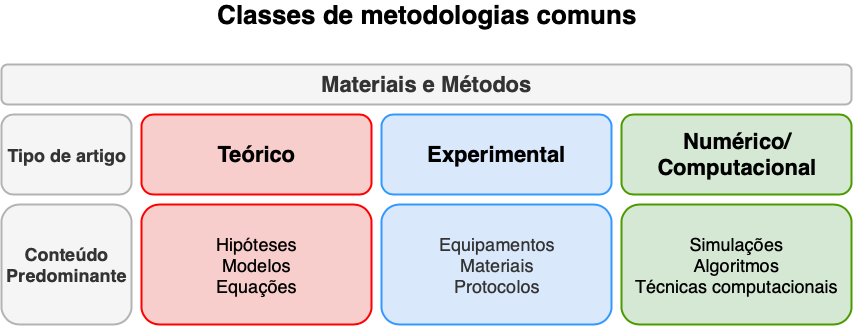
\includegraphics[scale=0.35]{figs/06/methods}
\caption{Fonte: Autor.}
\end{figure}
\end{frame}

\subsection{Características da seção}

\begin{frame}{Materiais}
\begin{itemize}
\item Especificações técnicas exatas 
\item Quantidades 
\item Fonte ou método de preparação
\item Propriedades físicas ou químicas 
\item Nomenclatura genérica ou química\footnote{Caso seja necessário citar marcas, o uso de símbolos específicos (\textcopyright, \textregistered, \texttrademark) pode ser obrigatório em determinados periódicos, mas não é tido como uma regra.} 
\end{itemize}
\end{frame}

%%
\begin{frame}{Métodos}
\begin{itemize}
\item Ordem usual é a cronológica
\item Inclua apenas informações essenciais
\item Especificidades técnicas podem ser movidas para apêndices ou suplementos 
\end{itemize}
\end{frame}

%%
\begin{frame}{Cabeçalhos}
\begin{itemize}
\item Subseções são geralmente usadas
\item Verifique artigos anteriores publicados na sua revista de interesse
\item Construa subseções que sejam consistentes com o que será apresentado como resultados 
\end{itemize}
\end{frame}

%%
\begin{frame}{Medições e análises}
\begin{itemize}
\item Encare como uma receita de bolo
\item Seja claro com quantidades e unidades de medida
\item ``Como'' e ``quanto''
\item Enfatize dados; não prolongue a descrição de analíses estatísticas
\item Métodos estatísticos ordinários devem ser usados sem comentários 
\item Métodos incomuns ou avançados devems ser referenciados 
\end{itemize}
\end{frame}

%%
\begin{frame}{Referências}
\begin{itemize}
\item Oriente o leitor a buscar informações detalhadas na literatura
\item Se seu método é novo, forneça todos os detalhes 
\item Se já tiver sido publicado, use a referência da literatura 
\item Métodos muito incomuns merecem uma explicação mínima
\end{itemize}
\end{frame}


%%
\begin{frame}{Tabelas e figuras}
\begin{itemize}
\item Listar propriedades e valores 
\item Ilustrar aparatos experimentais, processos, protocolos e/ou diagramas
\end{itemize}
\end{frame}


%% 
\begin{frame}{Forma e gramática}
\begin{itemize}
\item Não inclua resultados nesta seção
\item Informe o necessário para reprodutibilidade 
\item Seja rigoroso com a escrita nesta seção para evitar ambiguidades
\item O uso da voz passiva e o tempo passado podem ser predominantes
\end{itemize}
\end{frame}

\subsection{Exercício in-class}

%%
\begin{frame}{Tarefas}
\begin{enumerate}
\item Use os artigos da lista anterior para identificar seu tipo quanto à classe de materiais/métodos nele dispostos\footnote{A própria revista de publicação já deve dar um indicativo}
\item Tente identificar quais são os métodos, técnicas e/ou materiais citados para cada um
\end{enumerate}
\end{frame}

%% === REFS
\begin{frame}[allowframebreaks]
\frametitle{Referências}
\begin{thebibliography}{9}
\setbeamertemplate{bibliography item}[book]
%
\bibitem{ashby2005}Ashby, M. \textit{How to write a paper}. Engg. Dept., Univ. of Cambridge, 2005.
%
\bibitem{volpato2017}Volpato, G.L. \textit{Método Lógico para Redação Científica}. 2a. ed., Best Writing, 2017.
%
\bibitem{zuco2011}Zucolotto, V. \textit{Workshop de Capacitação em Escrita Científica}, Disponível em: \url{http://www.escritacientifica.sc.usp.br/escrita/cursos-escrita/}
%
\bibitem{day1993} Day, R. A., \textit{How to write and publish scientific papers}, Cambridge University Press, 1995.
\end{thebibliography}
\end{frame}